% Options for packages loaded elsewhere
\PassOptionsToPackage{unicode}{hyperref}
\PassOptionsToPackage{hyphens}{url}
%
\documentclass[
  letterpaper,
]{scrbook}

\usepackage{amsmath,amssymb}
\usepackage{iftex}
\ifPDFTeX
  \usepackage[T1]{fontenc}
  \usepackage[utf8]{inputenc}
  \usepackage{textcomp} % provide euro and other symbols
\else % if luatex or xetex
  \usepackage{unicode-math}
  \defaultfontfeatures{Scale=MatchLowercase}
  \defaultfontfeatures[\rmfamily]{Ligatures=TeX,Scale=1}
\fi
\usepackage{lmodern}
\ifPDFTeX\else  
    % xetex/luatex font selection
\fi
% Use upquote if available, for straight quotes in verbatim environments
\IfFileExists{upquote.sty}{\usepackage{upquote}}{}
\IfFileExists{microtype.sty}{% use microtype if available
  \usepackage[]{microtype}
  \UseMicrotypeSet[protrusion]{basicmath} % disable protrusion for tt fonts
}{}
\makeatletter
\@ifundefined{KOMAClassName}{% if non-KOMA class
  \IfFileExists{parskip.sty}{%
    \usepackage{parskip}
  }{% else
    \setlength{\parindent}{0pt}
    \setlength{\parskip}{6pt plus 2pt minus 1pt}}
}{% if KOMA class
  \KOMAoptions{parskip=half}}
\makeatother
\usepackage{xcolor}
\setlength{\emergencystretch}{3em} % prevent overfull lines
\setcounter{secnumdepth}{5}
% Make \paragraph and \subparagraph free-standing
\makeatletter
\ifx\paragraph\undefined\else
  \let\oldparagraph\paragraph
  \renewcommand{\paragraph}{
    \@ifstar
      \xxxParagraphStar
      \xxxParagraphNoStar
  }
  \newcommand{\xxxParagraphStar}[1]{\oldparagraph*{#1}\mbox{}}
  \newcommand{\xxxParagraphNoStar}[1]{\oldparagraph{#1}\mbox{}}
\fi
\ifx\subparagraph\undefined\else
  \let\oldsubparagraph\subparagraph
  \renewcommand{\subparagraph}{
    \@ifstar
      \xxxSubParagraphStar
      \xxxSubParagraphNoStar
  }
  \newcommand{\xxxSubParagraphStar}[1]{\oldsubparagraph*{#1}\mbox{}}
  \newcommand{\xxxSubParagraphNoStar}[1]{\oldsubparagraph{#1}\mbox{}}
\fi
\makeatother


\providecommand{\tightlist}{%
  \setlength{\itemsep}{0pt}\setlength{\parskip}{0pt}}\usepackage{longtable,booktabs,array}
\usepackage{calc} % for calculating minipage widths
% Correct order of tables after \paragraph or \subparagraph
\usepackage{etoolbox}
\makeatletter
\patchcmd\longtable{\par}{\if@noskipsec\mbox{}\fi\par}{}{}
\makeatother
% Allow footnotes in longtable head/foot
\IfFileExists{footnotehyper.sty}{\usepackage{footnotehyper}}{\usepackage{footnote}}
\makesavenoteenv{longtable}
\usepackage{graphicx}
\makeatletter
\newsavebox\pandoc@box
\newcommand*\pandocbounded[1]{% scales image to fit in text height/width
  \sbox\pandoc@box{#1}%
  \Gscale@div\@tempa{\textheight}{\dimexpr\ht\pandoc@box+\dp\pandoc@box\relax}%
  \Gscale@div\@tempb{\linewidth}{\wd\pandoc@box}%
  \ifdim\@tempb\p@<\@tempa\p@\let\@tempa\@tempb\fi% select the smaller of both
  \ifdim\@tempa\p@<\p@\scalebox{\@tempa}{\usebox\pandoc@box}%
  \else\usebox{\pandoc@box}%
  \fi%
}
% Set default figure placement to htbp
\def\fps@figure{htbp}
\makeatother
% definitions for citeproc citations
\NewDocumentCommand\citeproctext{}{}
\NewDocumentCommand\citeproc{mm}{%
  \begingroup\def\citeproctext{#2}\cite{#1}\endgroup}
\makeatletter
 % allow citations to break across lines
 \let\@cite@ofmt\@firstofone
 % avoid brackets around text for \cite:
 \def\@biblabel#1{}
 \def\@cite#1#2{{#1\if@tempswa , #2\fi}}
\makeatother
\newlength{\cslhangindent}
\setlength{\cslhangindent}{1.5em}
\newlength{\csllabelwidth}
\setlength{\csllabelwidth}{3em}
\newenvironment{CSLReferences}[2] % #1 hanging-indent, #2 entry-spacing
 {\begin{list}{}{%
  \setlength{\itemindent}{0pt}
  \setlength{\leftmargin}{0pt}
  \setlength{\parsep}{0pt}
  % turn on hanging indent if param 1 is 1
  \ifodd #1
   \setlength{\leftmargin}{\cslhangindent}
   \setlength{\itemindent}{-1\cslhangindent}
  \fi
  % set entry spacing
  \setlength{\itemsep}{#2\baselineskip}}}
 {\end{list}}
\usepackage{calc}
\newcommand{\CSLBlock}[1]{\hfill\break\parbox[t]{\linewidth}{\strut\ignorespaces#1\strut}}
\newcommand{\CSLLeftMargin}[1]{\parbox[t]{\csllabelwidth}{\strut#1\strut}}
\newcommand{\CSLRightInline}[1]{\parbox[t]{\linewidth - \csllabelwidth}{\strut#1\strut}}
\newcommand{\CSLIndent}[1]{\hspace{\cslhangindent}#1}

\makeatletter
\@ifpackageloaded{bookmark}{}{\usepackage{bookmark}}
\makeatother
\makeatletter
\@ifpackageloaded{caption}{}{\usepackage{caption}}
\AtBeginDocument{%
\ifdefined\contentsname
  \renewcommand*\contentsname{Table of contents}
\else
  \newcommand\contentsname{Table of contents}
\fi
\ifdefined\listfigurename
  \renewcommand*\listfigurename{List of Figures}
\else
  \newcommand\listfigurename{List of Figures}
\fi
\ifdefined\listtablename
  \renewcommand*\listtablename{List of Tables}
\else
  \newcommand\listtablename{List of Tables}
\fi
\ifdefined\figurename
  \renewcommand*\figurename{Figure}
\else
  \newcommand\figurename{Figure}
\fi
\ifdefined\tablename
  \renewcommand*\tablename{Table}
\else
  \newcommand\tablename{Table}
\fi
}
\@ifpackageloaded{float}{}{\usepackage{float}}
\floatstyle{ruled}
\@ifundefined{c@chapter}{\newfloat{codelisting}{h}{lop}}{\newfloat{codelisting}{h}{lop}[chapter]}
\floatname{codelisting}{Listing}
\newcommand*\listoflistings{\listof{codelisting}{List of Listings}}
\makeatother
\makeatletter
\makeatother
\makeatletter
\@ifpackageloaded{caption}{}{\usepackage{caption}}
\@ifpackageloaded{subcaption}{}{\usepackage{subcaption}}
\makeatother

\usepackage{bookmark}

\IfFileExists{xurl.sty}{\usepackage{xurl}}{} % add URL line breaks if available
\urlstyle{same} % disable monospaced font for URLs
\hypersetup{
  pdftitle={CASA0023 - Learning Diary},
  pdfauthor={Zhou Yingxi},
  hidelinks,
  pdfcreator={LaTeX via pandoc}}


\title{CASA0023 - Learning Diary}
\author{Zhou Yingxi}
\date{2025-03-28}

\begin{document}
\frontmatter
\maketitle

\renewcommand*\contentsname{Table of contents}
{
\setcounter{tocdepth}{2}
\tableofcontents
}

\mainmatter
\bookmarksetup{startatroot}

\chapter*{Welcome}\label{welcome}
\addcontentsline{toc}{chapter}{Welcome}

\markboth{Welcome}{Welcome}

Hi there! I'm Yingxi. On the following pages you'll find my learning
dairy for module CASA0023-Remote Sensing Cities and Environment ,
featured in the CASA, UCL, MSc program. For each week, you'll find a
short summary of some concepts covered that week, examples of how they
are applied, my learning outcomes and some personal reflections.

\bookmarksetup{startatroot}

\chapter{Getting started with Remote
sensing}\label{getting-started-with-remote-sensing}

\section{Summary}\label{summary}

\subsection{What is Remote Sensing?}\label{what-is-remote-sensing}

\begin{itemize}
\item
  Remote sensing is basically a way of collecting information about
  places or objects without physically being there.
\item
  It works by detecting energy (usually light or heat) that bounces off
  the Earth's surface.
\item
  Think of it like taking a photo from space, but with more than just
  visible light---some sensors can see heat, detect moisture, or even
  see through clouds!
\end{itemize}

\subsection{Types of Remote Sensing}\label{types-of-remote-sensing}

\begin{itemize}
\item
  Passive sensing → Relies on sunlight (like a regular camera, human
  eyes, satellite sensor).
\item
  Active sensing → Sends out its own signals and measures the response
  (like radar or LiDAR).
\end{itemize}

\subsection{Electromagnetic Radiation}\label{electromagnetic-radiation}

\begin{itemize}
\item
  Remote sensing works by detecting electromagnetic radiation (EMR),
  which includes visible light, infrared, and other types of waves.
\item
  Different surfaces reflect and absorb EMR differently, so we can use
  this to identify and analyze objects from a distance.
\item
  Different parts of the electromagnetic spectrum:
\end{itemize}

\pandocbounded{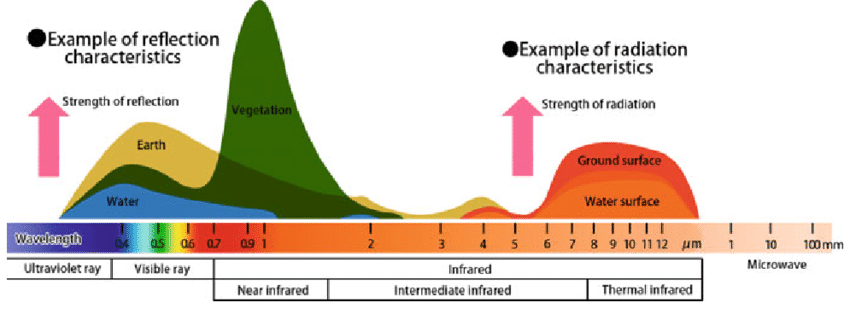
\includegraphics[keepaspectratio]{images/clipboard-1366391390.png}}

Figure 1 strength of reflection

Source:(Young and Onoda 2017)

\subsection{Resolution -- How clear is the
Image?}\label{resolution-how-clear-is-the-image}

\begin{itemize}
\item
  Spatial resolution -- How detailed an image is (higher resolution =
  smaller objects visible).
\item
  Temporal resolution -- How often images are taken (e.g., some
  satellites scan daily, others every few weeks).
\item
  Spectral resolution -- How many ``colors'' or wavelengths are detected
  (more bands = more data about the environment).
\item
  Radiometric resolution -- How precisely differences in energy levels
  are recorded (higher bit depth = more subtle variations detected).
\end{itemize}

\section{Applications}\label{applications}

In environmental monitoring, satellite remote sensing has emerged as a
cornerstone technology for tracking deforestation(Lima et al. 2019),
land-use changes (Frimpong and Molkenthin 2021), and ecological
degradation. The synergistic use of Sentinel-2 and Landsat systems
exemplifies the unique value of multi-scale Earth observation data in
ecological governance. The following are two different examples.

\begin{itemize}
\tightlist
\item
  Monitoring of Selective Logging in Tropical Forests
\end{itemize}

Lima et al.'s (2019) groundbreaking study on selective logging in the
Brazilian Amazon employed a self-referenced Normalized Burn Ratio index
through time-series analysis, revealing a critical paradox: while
Sentinel-2's 10-meter resolution better detected logging infrastructure
(43.2\% detection rate vs Landsat 8's 35.5\%), Landsat 8 captured 36.9\%
more disturbed area. This counterintuitive finding stems from Landsat's
broader spectral range enhancing sub-canopy disturbance sensitivity,
whereas Sentinel-2's high resolution, despite its precision, becomes
susceptible to canopy gap interference. The study's innovative 300m
assessment grid design effectively addressed mixed-pixel challenges
while aligning with local forestry management units, a methodology
subsequently adopted by Brazil's environmental agency for illegal
logging early-warning systems.

\pandocbounded{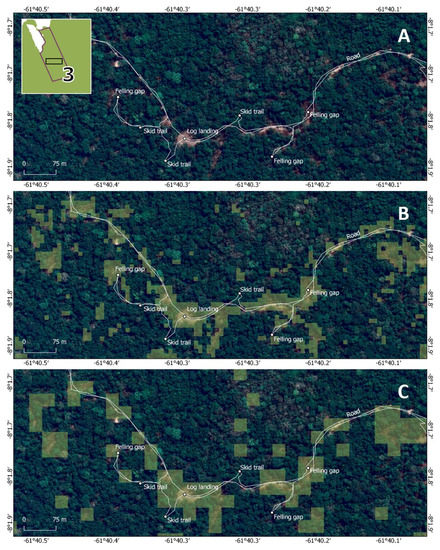
\includegraphics[keepaspectratio]{images/clipboard-2971102382.png}}

Figure 2 Detail of the sustainable forest management, showing: A) The
field data collected, B) Sentinel-2, and C) Landsat 8.

Source: Lima et al. (2019)

\begin{itemize}
\tightlist
\item
  Urban Expansion Analysis of Kumasi, Ghana
\end{itemize}

Frimpong and Molkenthin's (2021) longitudinal study of Kumasi, Ghana
demonstrates remote sensing's urban planning applications. By processing
1986-2015 Landsat imagery with Random Forest algorithms, the research
not only quantified the city's explosive growth from 23.78\% (1986) to
72.05\% (2015) urban coverage but also, through density decay curves,
revealed spatial heterogeneity in expansion patterns - particularly an
alarming 79.7\% agricultural land conversion rate in peri-urban zones.
The deliberate selection of Landsat over higher-resolution data proved
strategic: 30-meter resolution adequately captured West Africa's
characteristic clustered urban expansion patterns while leveraging
Landsat's unparalleled 40-year archive for longitudinal analysis.

\pandocbounded{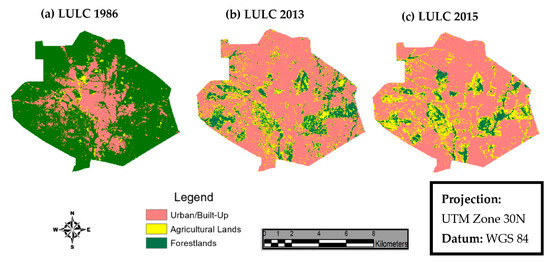
\includegraphics[keepaspectratio]{images/clipboard-1503754290.png}}

Figure 2 Land Use Land Cover (LULC) maps for the years 1986, 2013 and
2015

Source: Frimpong and Molkenthin (2021)

\section{Reflection}\label{reflection}

This lecture provided a clear introduction to remote sensing.It made me
have a general idea of how satellite imagery works, and let me realize
how different types of resolution determine what kind of information can
be extracted. For example, high temporal resolution is essential for
disaster monitoring, while high spectral resolution is better suited for
analyzing vegetation health. Understanding these differences helped me
see why different satellites are designed for specific applications.

One of the most interesting aspects was learning about the wide range of
applications. I was aware that remote sensing is used for weather
forecasting and mapping, but I hadn't considered its role in
agriculture, urban planning, and security. It was fascinating to see how
thermal infrared sensors detect wildfires in real-time, how radar
satellites track floods through cloud cover, and how spectral data can
reveal plant stress before it's visible.

I'm now curious about how satellite data is processed and analyzed. The
raw images must be converted into meaningful insights, often using GIS
and machine learning techniques. Moving forward, I want to learn more
about the analytical side of remote sensing and how it connects with my
research interests.

\section{Reference}\label{reference}

\bookmarksetup{startatroot}

\chapter{Xaringan}\label{xaringan}

Week 2 focused on the use of code to present and host websites and
slides, allowing for a portfolio to be formed. The task for week 2 is a
presentation in Xaringan on the \textbf{Sentinel-1 SAR} satellite.\\
The presentation is below, and the summary, application, and reflection
are all included in the slides.

\bookmarksetup{startatroot}

\chapter{Remote Sensing Data}\label{remote-sensing-data}

\section{Correction of Remote Sensing
Data}\label{correction-of-remote-sensing-data}

\subsection{Geometric Correction}\label{geometric-correction}

\begin{itemize}
\tightlist
\item
  \textbf{Problem}: Image positions don't match actual geographic
  locations
\item
  \textbf{Causes}:

  \begin{itemize}
  \tightlist
  \item
    Earth curvature effects
  \item
    Sensor viewing angle deviations
  \item
    Platform attitude variations (satellite/aircraft movement)
  \end{itemize}
\item
  \textbf{Correction Process}:

  \begin{itemize}
  \tightlist
  \item
    Ground Control Points (GCPs): Identify corresponding points between
    image and real ground
  \item
    Transformation Model: Calculate correction formulas (typically
    polynomial)
  \item
    Resampling: Assign values to new grid

    \begin{itemize}
    \tightlist
    \item
      Nearest Neighbor: Preserves original values, suitable for
      classified data
    \item
      Bilinear Interpolation: Averages values, produces smoother results
    \item
      Cubic Convolution: High quality but computationally intensive
    \end{itemize}
  \end{itemize}
\end{itemize}

\subsection{Atmospheric Correction}\label{atmospheric-correction}

\begin{itemize}
\tightlist
\item
  \textbf{Problem}: Atmospheric gases and particles interfere with
  signal transmission

  \begin{itemize}
  \tightlist
  \item
    Scattering: Changes light direction, increases path radiance
  \item
    Absorption: Weakens signal strength at specific wavelengths
  \end{itemize}
\item
  \textbf{Correction Methods}:

  \begin{itemize}
  \tightlist
  \item
    Dark Object Subtraction (DOS): Assumes brightness in dark areas
    comes from atmospheric scattering
  \item
    Radiative Transfer Code: Uses physical models to simulate and remove
    atmospheric effects
  \item
    Empirical Line Correction: Establishes empirical relationships using
    ground measurements
  \item
    Second-Order Derivative: Reduces background interference in spectral
    curves
  \end{itemize}
\item
  \textbf{Practical Advice}: DOS suitable for beginners, radiative
  transfer models recommended for professional analysis
\end{itemize}

\subsection{Orthorectification}\label{orthorectification}

\begin{itemize}
\tightlist
\item
  Special type of geometric correction that eliminates displacement
  caused by terrain
\item
  Requires DEM data to calculate actual position of each pixel
\item
  Generates orthoimages with uniform scale for direct measurement
\end{itemize}

\subsection{Reflectance Correction}\label{reflectance-correction}

\begin{itemize}
\tightlist
\item
  Conversion from Digital Numbers (DN) to physical values
\item
  Steps include:

  \begin{itemize}
  \tightlist
  \item
    Radiometric calibration: DN to radiance
  \item
    Top-of-Atmosphere (TOA) reflectance: Accounts for solar illumination
  \item
    Surface reflectance: After atmospheric correction
  \end{itemize}
\item
  Essential for quantitative analysis and multi-temporal comparisons
\end{itemize}

\subsection{Data Mosaicking}\label{data-mosaicking}

\begin{itemize}
\tightlist
\item
  Combines multiple images into a seamless large-area image
\item
  \textbf{Processing Steps}:

  \begin{itemize}
  \tightlist
  \item
    Precise registration of adjacent images
  \item
    Radiometric balancing to eliminate color differences
  \item
    Seamline optimization to avoid obvious features
  \item
    Edge blending to eliminate visible seams
  \end{itemize}
\end{itemize}

\section{Enhancement and Analysis of Remote Sensing
Data}\label{enhancement-and-analysis-of-remote-sensing-data}

\subsection{Image Enhancement
Techniques}\label{image-enhancement-techniques}

\begin{itemize}
\tightlist
\item
  \textbf{Contrast Stretching}: Expands histogram to enhance feature
  distinctiveness
\item
  \textbf{Filtering}:

  \begin{itemize}
  \tightlist
  \item
    Low-pass filters: Smooth noise
  \item
    High-pass filters: Enhance edges
  \end{itemize}
\item
  \textbf{Band Combinations}: Highlight specific features through
  different band combinations
\item
  \textbf{Principal Component Analysis (PCA)}: Dimension reduction while
  preserving key information
\item
  \textbf{Texture Analysis}: Extracts information about spatial
  arrangement patterns
\end{itemize}

\subsection{Remote Sensing Indices}\label{remote-sensing-indices}

\begin{itemize}
\tightlist
\item
  \textbf{Vegetation Indices}:

  \begin{itemize}
  \tightlist
  \item
    NDVI = (NIR-Red)/(NIR+Red): Reflects vegetation vigor
  \item
    EVI: Improved NDVI, reduces soil background effects
  \item
    SAVI: Suitable for areas with sparse vegetation
  \end{itemize}
\item
  \textbf{Water Indices}:

  \begin{itemize}
  \tightlist
  \item
    NDWI = (Green-NIR)/(Green+NIR): Extracts water bodies
  \item
    MNDWI: Improved version, reduces building interference
  \end{itemize}
\item
  \textbf{Built-up Indices}:

  \begin{itemize}
  \tightlist
  \item
    NDBI = (SWIR-NIR)/(SWIR+NIR): Highlights urban built-up areas
  \end{itemize}
\item
  \textbf{Other Thematic Indices}:

  \begin{itemize}
  \tightlist
  \item
    Soil indices, snow cover indices, drought indices, etc.
  \end{itemize}
\end{itemize}

\subsection{Image Classification
Methods}\label{image-classification-methods}

\begin{itemize}
\tightlist
\item
  \textbf{Supervised Classification}:

  \begin{itemize}
  \tightlist
  \item
    Requires training samples of known categories
  \item
    Algorithms: Maximum Likelihood, Support Vector Machine, Random
    Forest, Deep Learning
  \item
    Advantages: High accuracy, strong controllability
  \end{itemize}
\item
  \textbf{Unsupervised Classification}:

  \begin{itemize}
  \tightlist
  \item
    Automatic clustering, no prior knowledge needed
  \item
    Algorithms: K-means, ISODATA
  \item
    Advantages: Fast, suitable for preliminary analysis of unknown areas
  \end{itemize}
\item
  \textbf{Object-Based Classification}:

  \begin{itemize}
  \tightlist
  \item
    Segment first, then classify based on homogeneous regions
  \item
    Considers shape, texture, contextual relationships
  \item
    Suitable for high-resolution image analysis
  \end{itemize}
\end{itemize}

\subsection{Accuracy Assessment}\label{accuracy-assessment}

\begin{itemize}
\tightlist
\item
  \textbf{Error Matrix}: Compares predicted categories with reference
  data
\item
  \textbf{Evaluation Metrics}:

  \begin{itemize}
  \tightlist
  \item
    Overall Accuracy: Total proportion correctly classified
  \item
    User's Accuracy: Reliability of a classified category (reduces
    misclassification)
  \item
    Producer's Accuracy: Completeness of an actual category (reduces
    omission)
  \item
    Kappa Coefficient: Accounts for the possibility of random
    correctness
  \end{itemize}
\end{itemize}

\subsection{Change Detection
Techniques}\label{change-detection-techniques}

\begin{itemize}
\tightlist
\item
  \textbf{Image Differencing}: Direct calculation of multi-temporal
  image differences
\item
  \textbf{Ratio Analysis}: Calculates before/after ratios, reduces
  illumination effects
\item
  \textbf{Post-Classification Comparison}: Compares classification
  results from different periods
\item
  \textbf{Change Vector Analysis}: Direction and magnitude of changes
  across multiple bands
\end{itemize}

\bookmarksetup{startatroot}

\chapter{Applications}\label{applications-1}

Atmospheric correction (AC) is essential in ocean colour (OC) remote
sensing, as errors can significantly affect water reflectance retrieval.
Ilori et al. (2019) evaluated four AC methods for Landsat 8 OLI:
\textbf{ARCSI, ACOLITE, LaSRC, and SeaDAS}.

The study found that \textbf{ARCSI and LaSRC}, designed for land
applications, performed poorly over coastal waters, especially in the
\textbf{blue bands (e.g., 443 nm)}. In contrast, \textbf{ACOLITE and
SeaDAS}, optimized for aquatic environments, provided better accuracy.
Among them, \textbf{SeaDAS outperformed ACOLITE}, particularly in
complex waters, with lower root-mean-square errors (RMSE) ranging from
\textbf{0.0013 sr⁻¹ (443 nm) to 0.0005 sr⁻¹ (655 nm)}. Additionally,
\textbf{solar zenith angle and wind speed} significantly affected AC
errors for \textbf{ACOLITE and SeaDAS} in the 443 nm and 482 nm bands.

These findings are crucial for selecting appropriate AC methods for
\textbf{coastal and inland water monitoring}, improving the accuracy of
\textbf{water quality assessments, pollution detection, and climate
studies}. Further research is needed to validate AC methods in inland
and optically complex waters. As remote sensing advances, refining AC
algorithms will be essential for enhancing the accuracy of
high-resolution sensors like \textbf{Landsat 8 and Sentinel-2}.

\bookmarksetup{startatroot}

\chapter{Reflection}\label{reflection-1}

Learning about remote sensing data processing has fundamentally changed
my understanding of geospatial analysis. I now understand that raw data
contains numerous distortions and artifacts that must be systematically
addressed before meaningful analysis can begin. This realization has
instilled in me a deeper appreciation for the rigorous preprocessing
required for reliable results.

The systematic approach to data correction -- from geometric to
atmospheric to radiometric -- mirrors the scientific method itself,
requiring both theoretical understanding and practical implementation. I
found myself particularly intrigued by the trade-offs involved in
selecting correction methods. The choice between simplicity (like Dark
Object Subtraction) and sophistication (like radiative transfer models)
mirrors decisions I'll need to make in my own research, balancing
accuracy requirements against available resources and expertise.

This lecture has also highlighted the interdisciplinary nature of remote
sensing. The physics of atmospheric scattering, the mathematics of
transformation matrices, the computer science of image processing, and
the domain knowledge required for interpretation all converge in this
field. As someone interested in environmental applications, I now see
how essential these technical preprocessing steps are for generating
trustworthy analyses that can inform policy and management decisions.

\section{Reference}\label{reference-1}

\bookmarksetup{startatroot}

\chapter{Policy}\label{policy}

\section{Summary}\label{summary-1}

\textbf{Advantages of Using Remote Sensing in Policy}:

\begin{itemize}
\item
  Provides objective data at large scales and over long time series
\item
  Cost-effective, especially for inaccessible areas
\item
  Supports different stages of policy development
\item
  Data accuracy has significantly improved, particularly in the last 20
  years
\end{itemize}

\textbf{Key Policy Frameworks}: UN Sustainable Development Goals (SDGs);
UN Sendai Framework for Disaster Risk Reduction ; GEO (Group on Earth
Observations) working groups; Copernicus program (European)

\textbf{Remote Sensing Policy Application Examples}:

\begin{itemize}
\item
  Dujiangyan City light pollution study (night light data)
\item
  London tree canopy analysis (aerial and satellite data)
\item
  Climate change assessment and impacts
\item
  Urban planning and management
\item
  Disaster risk assessment (e.g., flood risk mapping)
\end{itemize}

\textbf{Challenges \& Limitations}:

\begin{itemize}
\item
  Data accessibility
\item
  Technical capacity requirements
\item
  Time delays and frequency issues
\item
  Communication barriers between decision
\item
  Need for integration with ground truth
\end{itemize}

\textbf{Policy Implementation Components}:

\begin{itemize}
\item
  Requires supporting enforcement and monitoring mechanisms
\item
  Integration of multi-source data for comprehensive analysis
\item
  Citizen participation and feedback
\item
  Policy evaluation and adjustment
\end{itemize}

\section{Applications}\label{applications-2}

Remote sensing is widely used in \textbf{ecological conservation and
natural resource management}. For instance, In the USA, Mayer and Lopez
(2011) argue that remote sensing has been instrumental in monitoring
forest and wetland conservation policies. For forests, remote sensing
aids in enforcing the ``Roadless Rule'' and ``Travel Management Rules''
by detecting unauthorized roads and trails in national forests.
High-resolution imagery, such as IKONOS and aerial photography, helps
identify ecological impacts of road fragmentation, guiding management
decisions to protect biodiversity and ecosystem services.

Also, remote sensing plays a vital role in \textbf{air pollution
monitoring}. Atmospheric remote sensing technologies, such as MODIS and
Sentinel-5P, provide aerosol optical depth (AOD) data to identify
pollution sources and inform mitigation strategies(Xue et al. 2017). In
China, high-resolution Gaofen satellites are used to monitor PM2.5
concentrations and integrate ground-based observations to enhance the
effectiveness of air pollution control policies like the ``Blue Sky
Protection Campaign.''

\section{Reflection}\label{reflection-2}

This lecture has provided me with valuable insights into how remote
sensing can be applied in policy-making, particularly in areas such as
environmental governance, urban planning, and disaster management. One
of the key takeaways is how satellite data, including SAR and optical
imagery, enables policymakers to make data-driven decisions rather than
relying on traditional, often outdated methods. For instance, I learned
that remote sensing plays a crucial role in monitoring forest and
wetland conservation policies and tracking air pollution. These
applications are essential for enforcing environmental policies and
meeting sustainability goals.

Another important aspect I learned from the lecture is the role of
remote sensing in disaster response and mitigation. By providing near
real-time data on earthquakes, floods, and wildfires, remote sensing
allows for rapid assessment of affected areas, improving emergency
response and resource allocation. This is particularly important in
climate adaptation policies, where data accuracy and timeliness are
critical.

Also, I think there are still some challenges in integrating remote
sensing into policy frameworks, such as data accessibility, processing
complexity, and ethical considerations related to privacy and
surveillance. I realized that while remote sensing offers powerful tools
for policy decision-making, its effectiveness depends on collaboration
between scientists, government agencies, and policymakers.

\section{Reference}\label{reference-2}

\bookmarksetup{startatroot}

\chapter{Google Earth Engine}\label{google-earth-engine}

\section{Summary}\label{summary-2}

Lecture 5 introduced Google Earth Engine (GEE), a powerful cloud
computing platform designed for processing and analyzing geospatial
data, particularly remote sensing data. GEE integrates vast geospatial
datasets with strong computational capabilities, enabling users to
efficiently process and analyze large-scale data.

\subsection{Advantages of GEE}\label{advantages-of-gee}

Data Storage and Access: Users can access and process data directly in
the cloud without downloading large datasets, saving local storage space
and improving efficiency.

Computational Power: Leveraging Google's robust infrastructure, GEE can
handle large-scale data processing, supporting complex analyses and
significantly reducing processing time.

Programming Interface: GEE offers both JavaScript and Python APIs,
allowing users to customize analysis workflows as needed. This
flexibility makes it suitable for various applications.

\subsection{Key Functions in GEE}\label{key-functions-in-gee}

Image Processing: Functions like ee.Image allow users to manipulate and
analyze satellite images, such as applying filters, enhancing contrast,
and extracting spectral indices (e.g., NDVI for vegetation analysis).

Data Collection and Filtering: ee.ImageCollection enables users to work
with large datasets, filtering by date, location, or cloud cover.

Geospatial Statistics: ee.Reducer functions help compute statistical
summaries (e.g., mean, median, min/max values) for specific regions.

Vector Data Processing: ee.Geometry and ee.FeatureCollection handle
vector data like points, lines, and polygons for spatial analysis.

\subsection{Essential Tools in GEE}\label{essential-tools-in-gee}

Code Editor: A powerful web-based IDE that allows users to write
JavaScript scripts, visualize data, and execute computations.

Asset Manager: Users can upload and manage their own datasets, such as
shapefiles or raster images.

Data Catalog: GEE provides access to extensive remote sensing and
geospatial datasets, including Landsat, Sentinel, MODIS, and global
climate models.

Map Visualization Tools: Users can overlay processed images, vector
data, and computed results onto interactive maps.

\section{Applications}\label{applications-3}

Google Earth Engine (GEE) has emerged as a transformative platform for
large-scale environmental monitoring.

Farhadi et al.(2025) developed an innovative Spectral Flood Mapping
Index (SFMI) using Sentinel-2 imagery within GEE, enabling automated
flood detection at 10-meter resolution. Their approach leverages GEE's
cloud computing power to process multi-temporal data and integrate
spectral indices (NDWI, NDVI) through Otsu's thresholding method,
significantly reducing processing time compared to traditional
workflows. This application is particularly valuable for disaster
response, where rapid flood mapping can inform emergency operations
within hours of data acquisition.

For long-term ecological assessment, Liu et al. (2023) utilized GEE to
analyze 40 years of Landsat imagery (1985-2022) for vegetation
monitoring on Zhoushan Island. The platform's ability to process over
5,000 Landsat scenes enabled comprehensive NDVI trend analysis,
revealing a 13\% decline in coastal vegetation. By incorporating spatial
statistics (Moran's I) and multivariate analysis of climate, terrain,
and anthropogenic factors, the study demonstrated GEE's capacity for
complex geospatial modeling at regional scales.

\pandocbounded{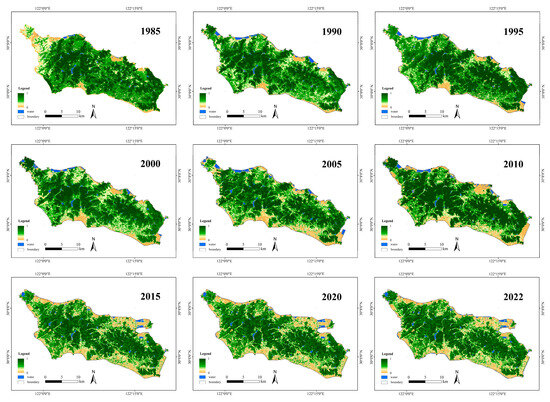
\includegraphics[keepaspectratio]{images/clipboard-1680012289.png}}

Fugire1: Spatiotemporal distribution maps of the NDVI on Zhoushan
Island from 1985 to 2022.

Source:Liu, Chen, and Chen (2023)

\section{Reflection}\label{reflection-3}

I found this session particularly insightful because it demonstrated how
large-scale geospatial analysis can be conducted efficiently without
requiring high-end hardware. The ability to access and process vast
datasets in the cloud is a significant advantage, especially for
environmental research, urban planning, and disaster management.

One key takeaway for me was how GEE integrates various datasets, such as
Landsat, Sentinel, and MODIS, into a single platform. This makes it much
easier to analyze long-term environmental changes without having to
manually collect and preprocess data. The fact that GEE provides
pre-processed and ready-to-use datasets greatly simplifies geospatial
analysis, which is particularly beneficial for beginners like me.

However, I also found the learning curve to be somewhat challenging.
Unlike traditional GIS software, which often has a graphical user
interface, GEE requires scripting in JavaScript or Python. Since I have
limited programming experience, writing scripts to filter datasets and
visualize results was initially difficult. So this lecture really
motivated me to improve my scripting abilities.

\section{Reference}\label{reference-3}

\bookmarksetup{startatroot}

\chapter{Classification I}\label{classification-i}

\section{Summary}\label{summary-3}

This lecture covered \textbf{classification methods} in remote sensing,
particularly \textbf{supervised and unsupervised classification}.
Classification is essential in spatial analysis as it helps extract
meaningful information from satellite imagery.

\subsection{\texorpdfstring{\textbf{Supervised
Classification}}{Supervised Classification}}\label{supervised-classification}

Supervised classification relies on labeled training data to categorize
pixels. Common methods include:

\begin{itemize}
\item
  \textbf{Maximum Likelihood Classification (MLC):} Assumes a normal
  distribution of data and assigns each pixel to the class with the
  highest probability.
\item
  \textbf{Support Vector Machines (SVM):} Identifies an optimal decision
  boundary between different classes.
\item
  \textbf{Random Forest (RF):} A machine learning approach using
  multiple decision trees for classification.
\end{itemize}

\subsection{\texorpdfstring{\textbf{Unsupervised
Classification}}{Unsupervised Classification}}\label{unsupervised-classification}

Unsupervised classification groups pixels into clusters based on
spectral properties without predefined labels. Common methods include:

\begin{itemize}
\item
  \textbf{K-Means Clustering:} Iteratively assigns pixels to K clusters
  by minimizing variance.
\item
  \textbf{ISODATA (Iterative Self-Organizing Data Analysis):} Allows
  merging and splitting of clusters for more flexibility.
\end{itemize}

This method is useful when ground truth data is unavailable, but class
labels must be assigned afterward.

\subsection{\texorpdfstring{\textbf{Mixed Pixels and
Challenges}}{Mixed Pixels and Challenges}}\label{mixed-pixels-and-challenges}

\begin{itemize}
\item
  \textbf{Mixed Pixels:} A single pixel may contain multiple land cover
  types, affecting classification accuracy.
\item
  \textbf{Solutions:} Spectral unmixing and increasing spatial
  resolution can help mitigate this issue.
\end{itemize}

\section{Applications}\label{applications-4}

Remote sensing classification have significantly enhanced land cover
mapping and environmental monitoring capabilities.

Kussul et al. (2017) developed an innovative deep learning framework
combining unsupervised and supervised neural networks for crop type
classification in Ukraine. Their multilevel architecture processes
multitemporal Landsat-8 and Sentinel-1A data, achieving over 85\%
accuracy in distinguishing five major crop types. The study demonstrated
CNNs' superior performance compared to traditional multilayer
perceptrons, particularly in differentiating spectrally similar crops
like maize and soybeans. The integrated unsupervised component
effectively handles cloud cover and missing data, while the supervised
ensemble improves classification robustness in heterogeneous
agricultural areas.

\pandocbounded{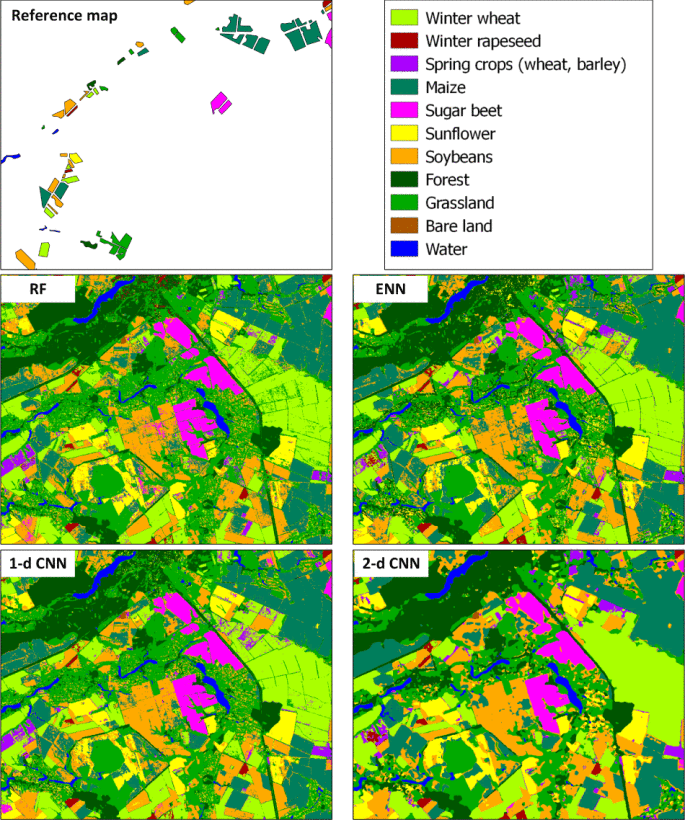
\includegraphics[keepaspectratio]{images/clipboard-2813045684.png}}

Figure 1 Example of classification result for the Kyiv region for 2015
based on all Landsat-8 and Sentinel-1A images

Source: Kussul et al. (2017)

Billah et al. (2023) implemented a random forest classifier for flood
damage assessment in northeast Bangladesh, utilizing combined Sentinel-1
and Sentinel-2 data. Their methodology achieved 90\% accuracy in land
cover classification, significantly outperforming conventional maximum
likelihood methods (74\% accuracy). The research highlighted SAR data's
value for reliable flood mapping during monsoons, complemented by
optical data for detailed land cover baselines. The study quantified
substantial agricultural impacts, with 23.98\% of cropland inundated
during monsoon floods and 72.41\% affected by flash floods, providing
critical data for disaster response planning in ecologically sensitive
wetland regions.

\pandocbounded{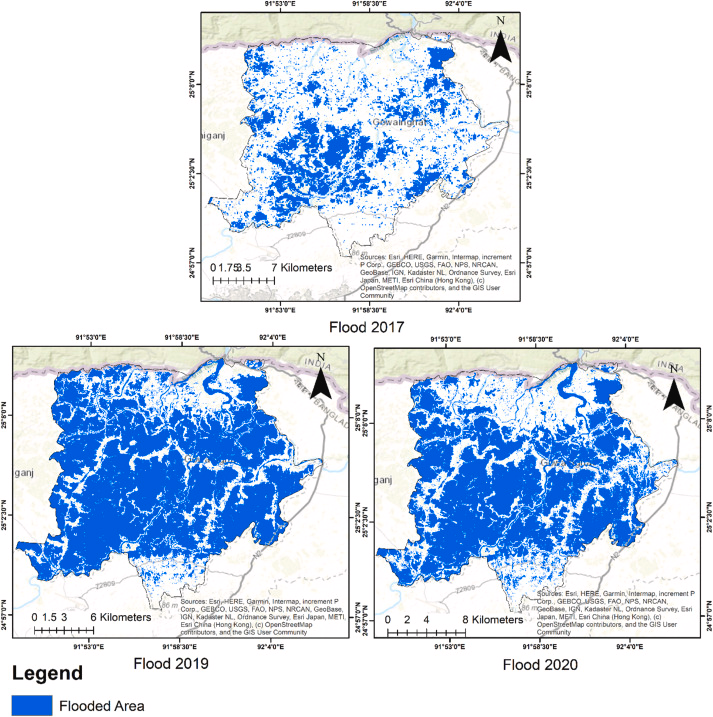
\includegraphics[keepaspectratio]{images/clipboard-1366614632.png}}

Figure 2 Flood maps for the early flood of 2017, flooding of 2019 and
severe flooding of 2020

Source: Billah et al. (2023)

\section{Reflection}\label{reflection-4}

This lecture deepened my understanding of classification techniques in
remote sensing, particularly the differences between supervised and
unsupervised approaches. I found it fascinating how these methods allow
us to extract valuable information from satellite imagery, helping
researchers analyze land use patterns, environmental changes, and
disaster impacts.

One aspect that stood out to me was the challenge of \textbf{mixed
pixels}, where a single pixel contains multiple land cover types. This
issue highlights the limitations of spatial resolution and the
importance of advanced techniques like spectral unmixing. It made me
think about how classification accuracy depends not only on the
algorithm but also on data quality, resolution, and preprocessing
methods.

The applications of classification in disaster management also intrigued
me. I had not fully realized the extent to which satellite-based
classification supports emergency response efforts, such as flood
mapping. This connects to my group research on Manchester's flooding
problem, where classification techniques could help analyze historical
flood patterns and identify high-risk areas.

\section{Reference}\label{reference-4}

\bookmarksetup{startatroot}

\chapter{Classification Ⅱ}\label{classification-ux2171}

\section{Summary}\label{summary-4}

\subsection{Classification
Methodologies}\label{classification-methodologies}

\subsubsection{Sub-Pixel Analysis}\label{sub-pixel-analysis}

Sub-pixel analysis addresses the complexity of pixels containing
multiple land cover types. Spectral Mixture Analysis (SMA) is a critical
technique that decomposes spectral reflectance within a pixel, precisely
calculating the proportion of different land covers. This method is
particularly useful for accurately classifying mixed pixels by
determining the exact contribution of each surface type.

\subsubsection{Object-Based Image Analysis
(OBIA)}\label{object-based-image-analysis-obia}

OBIA transcends traditional pixel-by-pixel classification by identifying
meaningful objects within pixel groups. The primary process involves:

\begin{itemize}
\item
  Image segmentation using algorithms like Simple Non-Iterative
  Clustering (SNIC)
\item
  Supervised or unsupervised classification of identified objects
\item
  Considering spectral and spatial characteristics of neighboring pixels
\end{itemize}

\subsubsection{Accuracy Assessment}\label{accuracy-assessment-1}

Accuracy assessment is the cornerstone of reliable remote sensing
classification:

\begin{itemize}
\item
  Producer's Accuracy: Percentage of classified samples matching ground
  truth data
\item
  User's Accuracy: Precision of sample matching between different
  classifications
\item
  Overall Accuracy: Percentage of correctly classified samples across
  all categories
\end{itemize}

\subsection{Advanced Validation
Techniques}\label{advanced-validation-techniques}

\subsubsection{Confusion Matrix}\label{confusion-matrix}

A critical tool for evaluating classification performance:

\begin{itemize}
\item
  Displays correct prediction scenarios
\item
  Analyzes omission and commission errors
\item
  Calculates Kappa coefficient to measure alignment between
  classification and labeled data
\end{itemize}

\subsubsection{Spatial Cross-Validation}\label{spatial-cross-validation}

Addressing spatial autocorrelation challenges:

\begin{itemize}
\item
  Prevents model overfitting
\item
  Ensures spatial independence of training and testing datasets
\item
  Mitigates overly optimistic accuracy estimations
\end{itemize}

\subsubsection{Receiver Operating Characteristic (ROC)
Curve}\label{receiver-operating-characteristic-roc-curve}

Graphically represents classification model performance by plotting true
positive rates against false positive rates, enabling simultaneous
evaluation of multiple classification models.

\section{Applications}\label{applications-5}

Remote sensing classification techniques extend beyond traditional
environmental and urban applications, they also play a crucial role in
fields such as public health, archaeology, and military intelligence. By
leveraging high-resolution imagery and machine learning algorithms,
researchers can extract valuable insights that support various
scientific and strategic objectives.

\subsection{\texorpdfstring{\textbf{Epidemiology and Public
Health}}{Epidemiology and Public Health}}\label{epidemiology-and-public-health}

Satellite-based classification has proven useful in tracking disease
outbreaks and environmental factors influencing public health. For
instance, remote sensing is used to classify land cover changes
associated with vector-borne diseases like malaria and dengue. By
identifying stagnant water bodies and deforested areas, health
authorities can predict mosquito breeding grounds and improve disease
prevention strategies. Additionally, air quality assessments rely on
classification to detect pollution hotspots, aiding in respiratory
disease mitigation efforts.

\subsection{\texorpdfstring{\textbf{Archaeological Site
Detection}}{Archaeological Site Detection}}\label{archaeological-site-detection}

Advanced classification techniques, including Object-Based Image
Analysis (OBIA), are revolutionizing archaeological studies. By
analyzing soil composition, vegetation patterns, and thermal anomalies,
researchers can identify buried structures and ancient settlements
without excavation. For example, classified satellite images have
revealed lost cities in dense rainforests, where conventional survey
methods are impractical.

\subsection{\texorpdfstring{\textbf{Military and Defense
Applications}}{Military and Defense Applications}}\label{military-and-defense-applications}

In defense and intelligence, classification plays a critical role in
monitoring geopolitical changes. High-resolution satellite imagery is
classified to detect military installations, track troop movements, and
assess terrain conditions. Synthetic Aperture Radar (SAR)-based
classification is particularly valuable in detecting hidden structures
and distinguishing between natural and artificial objects, even under
cloud cover.

\subsection{\texorpdfstring{\textbf{Space Exploration and Planetary
Mapping}}{Space Exploration and Planetary Mapping}}\label{space-exploration-and-planetary-mapping}

Remote sensing classification is instrumental in analyzing
extraterrestrial landscapes. NASA and ESA use classification models to
map Martian surface compositions, identifying features such as ice
deposits, volcanic plains, and ancient riverbeds. These insights guide
rover missions and future colonization efforts by determining suitable
landing sites and resource availability.

\subsection{\texorpdfstring{\textbf{Fisheries and Marine Ecosystem
Monitoring}}{Fisheries and Marine Ecosystem Monitoring}}\label{fisheries-and-marine-ecosystem-monitoring}

Beyond terrestrial applications, classification techniques are widely
applied in marine studies. Satellite imagery helps identify harmful
algal blooms (HABs) that threaten marine biodiversity and human health.
Additionally, ocean surface classification supports sustainable
fisheries management by tracking fish migration patterns and detecting
illegal fishing activities.

\section{Reflection}\label{reflection-5}

This lecture deepened my understanding of remote sensing classification
techniques and their practical applications, particularly in disaster
management. The discussion on \textbf{sub-pixel analysis} and
\textbf{object-based image analysis (OBIA)} highlighted their advantages
in capturing complex land cover variations, which is relevant to my
group project on \textbf{flood detection in Manchester}. Given
Manchester's susceptibility to flooding, accurately classifying
\textbf{flooded areas in urban environments} is critical for effective
response and resilience planning.

One key insight was the \textbf{importance of high-resolution
classification} in flood mapping. Traditional pixel-based approaches
often misclassify urban water accumulation, while OBIA allows for
\textbf{spatially aware segmentation}, distinguishing between
\textbf{flooded roads, waterlogged parks, and unaffected surfaces}.
Applying OBIA to \textbf{Sentinel-2 or Landsat imagery} in our project
could enhance flood risk assessments by improving classification
accuracy.

The role of \textbf{machine learning models}, such as
\textbf{Convolutional Neural Networks (CNNs)}, in land cover
classification was another crucial takeaway. The \textbf{Dynamic World
approach}, which leverages near real-time Sentinel-2 data, demonstrated
how \textbf{semi-supervised classification} can improve flood detection.
Integrating CNN-based classification with \textbf{Manchester's
historical flood data and real-time weather inputs} could enhance early
warning systems.

Lastly, the discussion on \textbf{spatial cross-validation} was
particularly relevant. Overfitting to past flood events is a risk when
training classification models, especially in urban environments where
land cover characteristics change over time. Ensuring that our
classification model \textbf{generalizes well to future flood events}
will be critical for our project's success.

Overall, this lecture provided valuable insights that we can apply to
our group work. By refining flood detection models using
\textbf{advanced classification techniques, machine learning, and
real-time satellite data}, we aim to develop a more effective approach
to monitoring and mitigating Manchester's flood risks.

\bookmarksetup{startatroot}

\chapter{SAR}\label{sar}

\section{Summary}\label{summary-5}

\subsection{Technical Characteristics}\label{technical-characteristics}

SAR is an active remote sensing sensor that simultaneously records two
critical types of data:

\begin{itemize}
\item
  Amplitude (backscatter)
\item
  Phase data (wave cycle location)
\end{itemize}

\subsection{Key Analytical
Considerations}\label{key-analytical-considerations}

\begin{enumerate}
\def\labelenumi{\arabic{enumi}.}
\item
  Polarization

  \begin{itemize}
  \item
    Different polarizations (e.g., VV) reveal surface roughness
    characteristics
  \item
    Provides insights into surface material properties
  \end{itemize}
\item
  Permativity (Dielectric Constant)

  \begin{itemize}
  \item
    Indicates the material's reflectivity back to the sensor
  \item
    Varies across different surface types
  \item
    Water tends to reflect signals away from the sensor
  \end{itemize}
\item
  Wavelength
\end{enumerate}

\begin{itemize}
\tightlist
\item
  Different bands provide varied surface interaction information
\end{itemize}

\section{Data Representation in Google Earth
Engine}\label{data-representation-in-google-earth-engine}

\begin{itemize}
\item
  Limited to amplitude (backscatter) data
\item
  Three primary data units:

  \begin{enumerate}
  \def\labelenumi{\arabic{enumi}.}
  \item
    Power scale: Raw SAR data for statistical analysis
  \item
    Amplitude: Visualization purposes
  \item
    Decibel (dB) scale: Highlighting differences (default in GEE)
  \end{enumerate}
\end{itemize}

\subsection{Unique Advantages and Analysis
Techniques}\label{unique-advantages-and-analysis-techniques}

\subsubsection{Distinctive Sensor
Capabilities}\label{distinctive-sensor-capabilities}

\begin{itemize}
\tightlist
\item
  Penetrates cloud cover
\item
  Operates independently of optical sensor limitations
\end{itemize}

\subsubsection{Analysis Methods}\label{analysis-methods}

\begin{enumerate}
\def\labelenumi{\arabic{enumi}.}
\item
  Change Detection

  \begin{itemize}
  \tightlist
  \item
    Comparing images using ratio or log ratio techniques
  \end{itemize}
\item
  Temporal Analysis

  \begin{itemize}
  \item
    T-tests
  \item
    Standard deviation calculations
  \item
    Exploring variance over time
  \end{itemize}
\item
  Data Fusion Techniques

  \begin{itemize}
  \item
    Principal Component Analysis
  \item
    Object-Based Image Analysis
  \item
    Intensity fusion with optical data
  \end{itemize}
\end{enumerate}

\subsubsection{1.SAR fundamentals}\label{sar-fundamentals}

SAR: Different surfaces respond differently to the polarizations A SAR
signal has both amplitude (backscatter) and phase data. different
weather show different signal: windy day-the surface of the water is
rough

InSAR: combine two or more SAR image DInSAR: remove the effet of natural
elevtation (DSM/DEM/DTM)

\subsection{2. GEE SAR}\label{gee-sar}

SAR data values: identify changes: substract image is not suitable for
SAR Ratio images: IR(improved ratio);mean; log; IRL(improved log ratio)
which is best and how to test them?

\section{Applications}\label{applications-6}

\subsection{Agricultural Monitoring and Crop
Management}\label{agricultural-monitoring-and-crop-management}

SAR technology offers unprecedented capabilities in agricultural
research and monitoring. Unlike optical sensors constrained by cloud
cover and daylight limitations, SAR can consistently track agricultural
landscapes throughout the year. By analyzing backscatter signals,
researchers can extract critical information about crop health, growth
stages, and land use patterns.

The technology enables precise monitoring of crop conditions by
detecting changes in surface roughness and moisture content. Different
polarization modes allow scientists to distinguish between various crop
types, assess vegetation density, and predict potential yield. For
instance, winter wheat fields exhibit distinct backscatter signatures
during different growth stages, enabling early detection of potential
crop stress or disease.

Flood and moisture mapping represent another crucial agricultural
application. SAR's ability to penetrate cloud cover and measure surface
moisture makes it invaluable for tracking potential agricultural risks.
Farmers and policymakers can use these insights to predict irrigation
needs, assess flood damage, and develop more resilient agricultural
strategies.

\subsection{Disaster Risk and Environmental
Management}\label{disaster-risk-and-environmental-management}

In disaster management, SAR provides critical real-time monitoring
capabilities that traditional remote sensing techniques cannot match.
The technology's ability to generate consistent imagery through adverse
weather conditions makes it exceptionally valuable for tracking dynamic
environmental changes.

Earthquake and landslide risk assessment benefit significantly from SAR
interferometry. By comparing multiple SAR images of the same location
over time, researchers can detect minute ground surface movements as
small as millimeters. This capability allows for early warning systems
in tectonically active regions, potentially saving lives and mitigating
infrastructure damage.

Additionally, SAR plays a crucial role in monitoring environmental
phenomena like deforestation, urban expansion, and coastal changes. Its
capacity to provide detailed surface information regardless of
atmospheric conditions enables comprehensive environmental surveillance.
Scientists can track forest cover changes, monitor sea-level rise, and
assess infrastructure development with unprecedented precision.

\section{Reflection}\label{reflection-6}

Before this lecture, I already had a general understanding of
\textbf{how SAR works}, but my knowledge was mostly theoretical. What I
hadn't fully grasped were its \textbf{practical advantages for flood
detection} and the specific \textbf{data processing techniques} required
to extract meaningful insights. The lecture clarified why SAR is so
effective in flood monitoring---not just because of its
\textbf{cloud-penetrating ability}, but also due to its
\textbf{sensitivity to surface water through backscatter variations}. I
found the discussion on \textbf{VV vs.~VH polarization} particularly
useful, as it explained why VV polarization is more responsive to open
water, influencing how we selected data for our group project.

Initially, our approach to \textbf{flood detection in Manchester} was
centered on optical data. While we were aware of SAR's potential, we
hadn't fully considered the practical challenges of working with
\textbf{speckle noise and change detection methods}. The lecture
introduced us to techniques like the \textbf{Improved Log Ratio (IRL)},
which proved more effective than simple subtraction when analyzing flood
extent. Another key takeaway was how \textbf{dielectric properties
influence SAR backscatter}, helping us interpret unexpected patterns,
such as \textbf{higher returns from flooded vegetation} due to
double-bounce effects.

Moving forward, I see value in integrating \textbf{SAR and optical data}
for a more comprehensive flood analysis and potentially incorporating
\textbf{InSAR techniques to monitor flood-induced land deformation}. The
lecture not only refined our group project's methodology but also
deepened my appreciation for the complexities of \textbf{SAR data
processing} in real-world applications.

\section*{Reference}\label{reference-5}
\addcontentsline{toc}{section}{Reference}

\phantomsection\label{refs}
\begin{CSLReferences}{1}{0}
\bibitem[\citeproctext]{ref-billah2023random}
Billah, Maruf, A. K. M. Saiful Islam, Wasif Bin Mamoon, and Mohammad
Rezaur Rahman. 2023. {``Random Forest Classifications for Landuse
Mapping to Assess Rapid Flood Damage Using {Sentinel-1} and {Sentinel-2}
Data.''} \emph{Remote Sensing Applications: Society and Environment} 30:
100947. \url{https://doi.org/10.1016/j.rsase.2023.100947}.

\bibitem[\citeproctext]{ref-farhadi2025introducing}
Farhadi, Hadi, Hamid Ebadi, Abbas Kiani, and Ali Asgary. 2025.
{``Introducing a New Index for Flood Mapping Using {Sentinel-2} Imagery
({SFMI}).''} \emph{Computers \& Geosciences} 194: 105742.
\url{https://doi.org/10.1016/j.cageo.2024.105742}.

\bibitem[\citeproctext]{ref-frimpong2021tracking}
Frimpong, Bismark Kwasi, and Frank Molkenthin. 2021. {``Tracking Urban
Expansion Using Random Forests for the Classification of Landsat Imagery
(1986--2015) and Predicting Urban/Built-up Areas for 2025: A Study of
the Kumasi Metropolis, Ghana.''} \emph{Land} 10 (1): 44.
\url{https://doi.org/10.3390/land10010044}.

\bibitem[\citeproctext]{ref-ilori2019analyzing}
Ilori, Christopher O., Nima Pahlevan, and Anders Knudby. 2019.
{``Analyzing Performances of Different Atmospheric Correction Techniques
for {Landsat} 8: Application for Coastal Remote Sensing.''} \emph{Remote
Sensing} 11 (4): 469. \url{https://doi.org/10.3390/rs11040469}.

\bibitem[\citeproctext]{ref-kussul2017deep}
Kussul, Nataliia, Mykola Lavreniuk, Sergii Skakun, and Andrii Shelestov.
2017. {``Deep Learning Classification of Land Cover and Crop Types Using
Remote Sensing Data.''} \emph{IEEE Geoscience and Remote Sensing
Letters} 14 (5): 778--82.
\url{https://doi.org/10.1109/LGRS.2017.2681128}.

\bibitem[\citeproctext]{ref-lima2019comparing}
Lima, Taise A., Rémi Beuchle, Andreas Langner, et al. 2019. {``Comparing
Sentinel-2 MSI and Landsat 8 OLI Imagery for Monitoring Selective
Logging in the Brazilian Amazon.''} \emph{Remote Sensing} 11 (8): 961.
\url{https://doi.org/10.3390/rs11080961}.

\bibitem[\citeproctext]{ref-liu2023analysis}
Liu, Zheng, Yang Chen, and Cheng Chen. 2023. {``Analysis of the
Spatiotemporal Characteristics and Influencing Factors of the {NDVI}
Based on the {GEE} Cloud Platform and {Landsat} Images.''} \emph{Remote
Sensing} 15 (20): 4980. \url{https://doi.org/10.3390/rs15204980}.

\bibitem[\citeproctext]{ref-mayer2011remote}
Mayer, Audrey L., and Ricardo D. Lopez. 2011. {``Use of Remote Sensing
to Support Forest and Wetlands Policies in the {USA}.''} \emph{Remote
Sensing} 3 (6): 1211--33. \url{https://doi.org/10.3390/rs3061211}.

\bibitem[\citeproctext]{ref-xue2017fusing}
Xue, Tao, Yixuan Zheng, Guannan Geng, Bo Zheng, Xujia Jiang, Qiang
Zhang, and Kebin He. 2017. {``Fusing Observational, Satellite Remote
Sensing and Air Quality Model Simulated Data to Estimate Spatiotemporal
Variations of {PM2}.5 Exposure in {China}.''} \emph{Remote Sensing} 9
(3): 221. \url{https://doi.org/10.3390/rs9030221}.

\bibitem[\citeproctext]{ref-young2017satellite}
Young, Oran, and Masami Onoda. 2017. {``Satellite Earth Observations in
Environmental Problem-Solving.''} In \emph{Satellite Earth Observations
and Their Impact on Society and Policy}, 3--27. Springer.

\end{CSLReferences}


\backmatter


\end{document}
